\documentclass[]{article}
\usepackage[T1]{fontenc}
\usepackage[utf8]{inputenc}
\usepackage[english]{babel}
%\usepackage[swedish]{babel}
\usepackage[toc,page]{appendix}
\usepackage{tikz, tkz-euclide}
\usepackage{textgreek}
\usepackage{blindtext}
\usepackage{circuitikz}
\usetikzlibrary{arrows}
\usepackage{siunitx}
\usepackage{geometry}
\usepackage{lipsum}
\usepackage{siunitx}
\usepackage{verbatim}
\usepackage{subcaption}
\usepackage{amsmath}
\usepackage{bm}
\usepackage{physics}
\usepackage{graphicx}%package to manage images
\graphicspath{{images/}}
\usepackage{wrapfig}
\usepackage{placeins}
\usepackage{graphicx}
\usepackage{caption}
\usepackage{authblk}
\usepackage{etoolbox}
\usepackage{lmodern}
\usepackage{amssymb}
\usepackage{float}

\newcommand{\uvec}[1]{\boldsymbol{\hat{\textbf{#1}}}}

\begin{comment}
    \usepackage{amssymb}
    \usepackage{enumerate}
    \usepackage{array}
    \usepackage{mathrsfs}
    \usepackage{tikz}
    \addto\captionsswedish{
        \renewcommand\appendixname{Bilaga}
        \renewcommand\appendixpagename{Bilaga}
        \renewcommand\appendixtocname{Bilaga}
    }
    \tikzset{node distance=2cm, auto}
    \usetikzlibrary{arrows}
    \allowdisplaybreaks
\end{comment}

\begin{document}

\newcommand{\uvec}[1]{\boldsymbol{\hat{\textbf{#1}}}}

\begin{comment}
    \usepackage{amssymb}
    \usepackage{enumerate}
    \usepackage{array}
    \usepackage{mathrsfs}
    \usepackage{tikz}
    \addto\captionsswedish{
        \renewcommand\appendixname{Bilaga}
        \renewcommand\appendixpagename{Bilaga}
        \renewcommand\appendixtocname{Bilaga}
    }
    \tikzset{node distance=2cm, auto}
    \usetikzlibrary{arrows}
    \allowdisplaybreaks
\end{comment}

\makeatletter
\patchcmd{\@maketitle}{\LARGE \@title}{\fontsize{16}{19.2}\selectfont\@title}{}{}
\makeatother

\renewcommand\Authfont{\fontsize{12}{14.4}\selectfont}
\renewcommand\Affilfont{\fontsize{9}{10.8}\itshape}
\begin{titlepage}
		\centering
		
\includegraphics[width=0.3\textwidth]{logo}\par\vspace{1cm}
		{\scshape\LARGE Lund's University \par}
		{\scshape\large The Faculty of Science, 
Department of Mathematics\par}
		\vspace{0.2cm}
		{\huge\bfseries MNXB01 Project Report, Group F\par}
		\vspace{2cm}
		{\Large\itshape Paulina Benthem Ciano, Dustin Lindner Daii,\\ Edmund Lehsten, Anton Palets \par}
		{\scshape Course: MNXB01}
		\par
		\vfill
	   
		
		\vfill
		
		% Bottom of the page
		{\large \today\par}
	\end{titlepage}
	\newpage
	\newpage
	\title{}
\newpage

\tableofcontents
\newpage

\section{Intro}

In this project we were given data from SMHI to write a program which extracts climate data from Sweden. After cleaning the data we make use of ROOT to create plots and perform some statistical analysis. There are three primary results which we study. The first is the temperature of a given day, we then expand upon this to see the temperature for every day of the year rather than one day. Finally, we investigate the covariance between the weather in Lund and Falsterbo as well as the covariance in Lund and Umeå and see what conclusions can be drawn. 

\section{Temperature of a given day}

Following the first example in the project instructions, the goal of this exercise is to calculate the histogram of the temperature of a given day, the mean temperature of that given day and the standard deviation of the temperature. The function \texttt{tempOnDay} can take as input either the date by month and day, or the day of the year. The histogram gets filled with the temperature of the given day over all years with available data. 

In Figure 1, the resulting histogram for input date (8/23) is presented. The probability of observing a particular temperature on a given day can be calculated by the number of entries in the histogram for the particular temperature divided by the total number of entries.

\begin{figure}[h]
    \centering
    \begin{subfigure}[b]{0.49\textwidth}
    \centering
    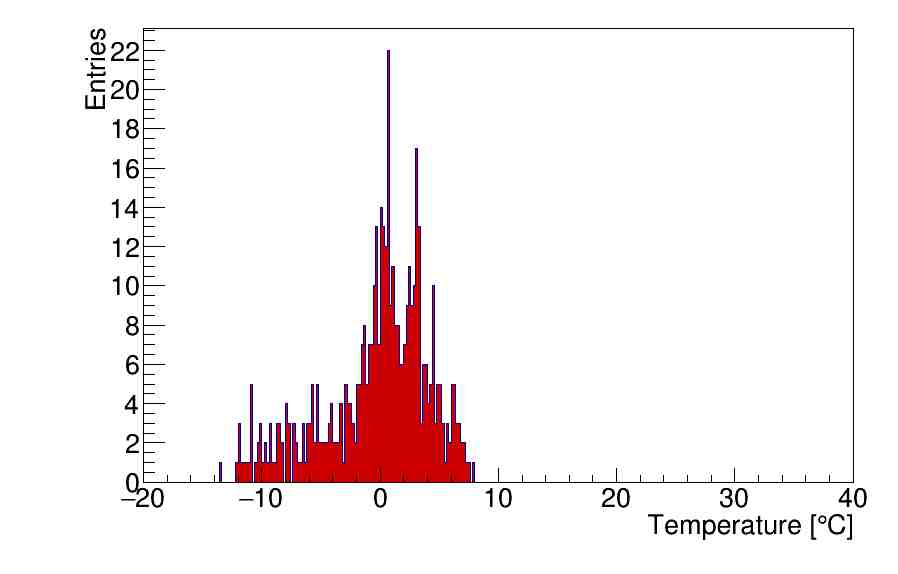
\includegraphics[width=\textwidth]{LU_1_P.jpg}
        \caption{Falsterbo}
    \end{subfigure}
    \hfill
    \begin{subfigure}[b]{0.49\textwidth}
    \centering
    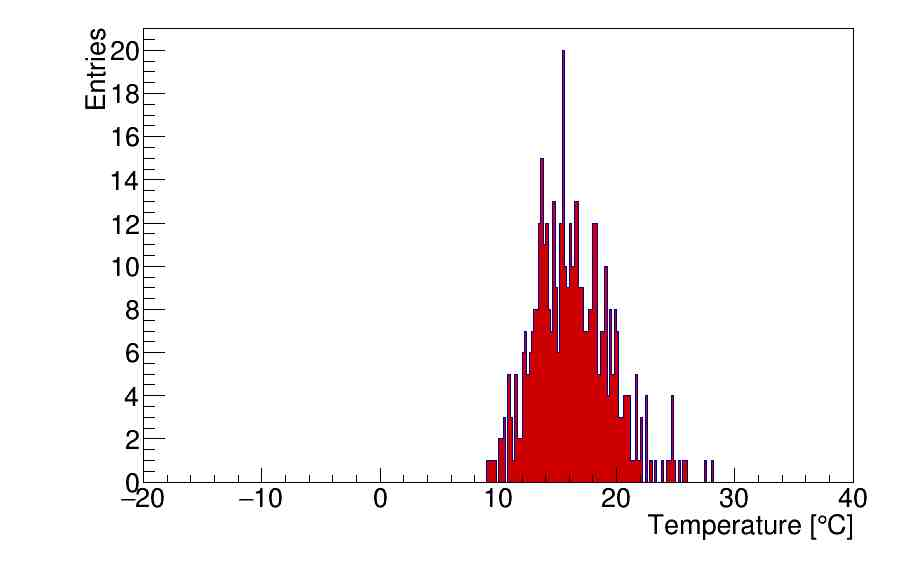
\includegraphics[width=\textwidth]{LU_8_23_P.jpg}
        \caption{Göteborg}
    \end{subfigure}
    
\end{figure}






\section{The temperature for every day of the year}

%Part 3.2

To see the average trend of temperature throughout the year, we can average out the temperature for each date and add it to a histogram. The way this is implemented is by using a while loop that goes line by line of cleaned up .csv file. Within the while loop we check whether the current line has the same date as the previous, and if so we add the temperature to the running total, if not we find the mean of the previous running total and add it to the correct bin of the histogram. Due to this implementation, the last group of entries will not be added to the histogram, as the while loop would have to run again, but this is easy to fix because the necessary information is still stored in the variables. We address this by adding the last group of entries to the histogram outside the loop. Since all the mean temperatures are added to the bins, we need to then normalize the bin values by the number of weighted entries. We create a normalization array and in it count how many times a day was added to the histogram. See the plots in the Figures section. One can see that the climate is milder in cities that are not on or close to the coast. For example, it might be that Kiruna has the biggest spread of temperatures because the presence of mountains generally makes the weather harsher. 

\begin{table}[h]
    \centering
    \begin{tabular}{|c|c|c|} \hline
        City  & Max & Min \\ \hline
        Lund & 14.3896 & 1.35988 \\
        Falsterbo & 15.2263 & 1.98313 \\
        Kiruna & 13.4096 & -14.0109 \\
        Göteborg & 14.6356 & 1.43963 \\
        Gävle & 13.8721 & -2.83569 \\
        Jönköping & 12.6589 & -0.163235 \\
        \hline
        
    \end{tabular}
    \caption{Maximum and minimum mean temperatures in different cities}
    \label{tab:my_label}
\end{table}

\begin{figure}
    \centering
    \begin{subfigure}[b]{0.49\textwidth}
    \centering
    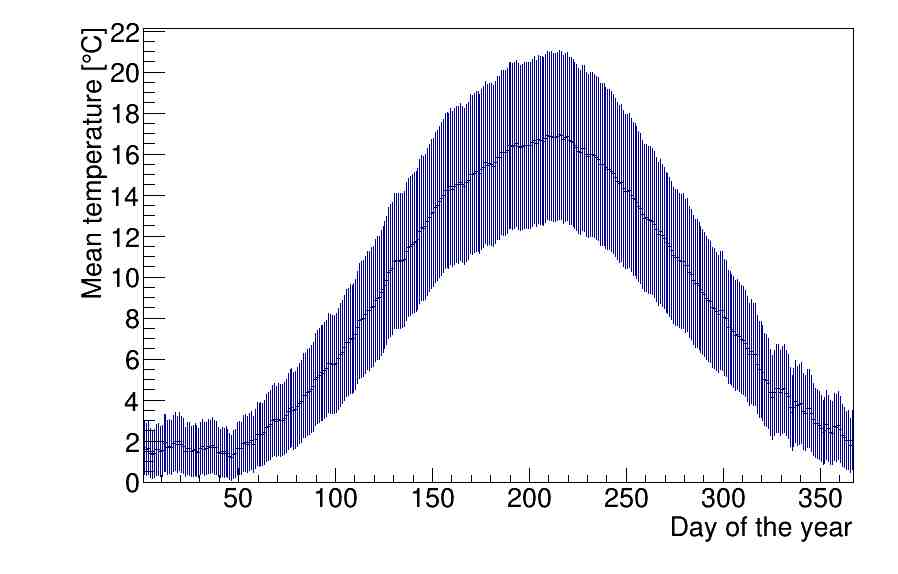
\includegraphics[width=\textwidth]{FAL_A.jpg}
        \caption{Falsterbo}
    \end{subfigure}
    \hfill
    \begin{subfigure}[b]{0.49\textwidth}
    \centering
    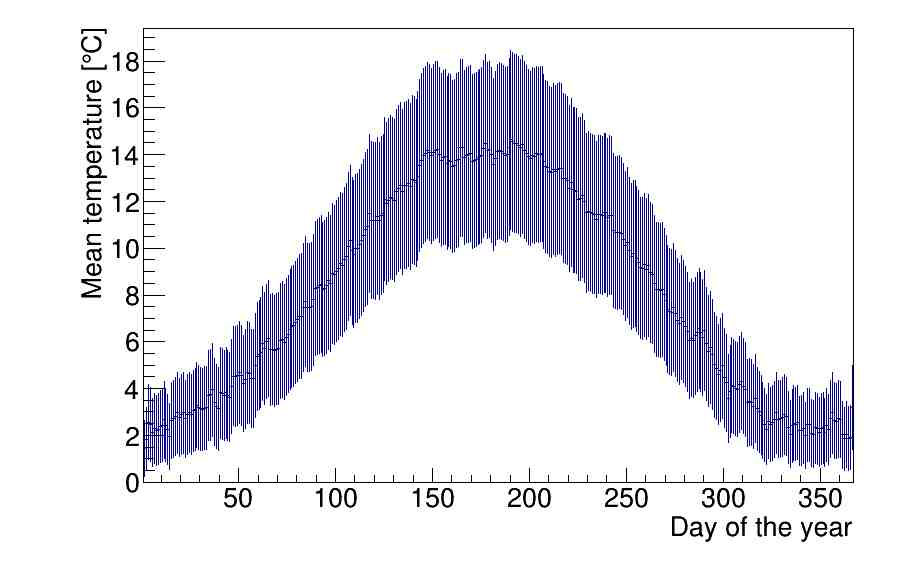
\includegraphics[width=\textwidth]{GBG_A.jpg}
        \caption{Göteborg}
    \end{subfigure}
    
    \begin{subfigure}[b]{0.49\textwidth}
    \centering
    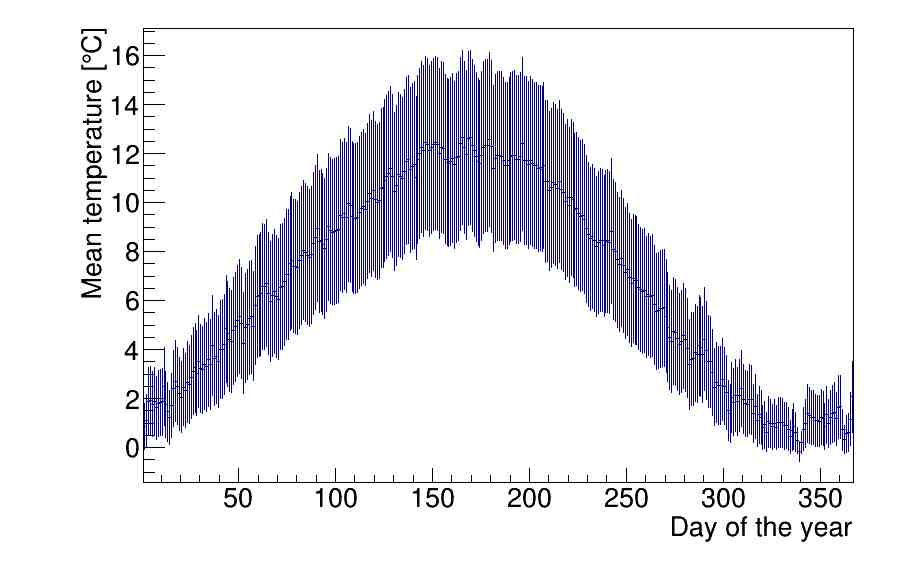
\includegraphics[width=\textwidth]{JKP_A.jpg}
        \caption{Jönköping}
    \end{subfigure}
    \hfill
    \begin{subfigure}[b]{0.49\textwidth}
    \centering
    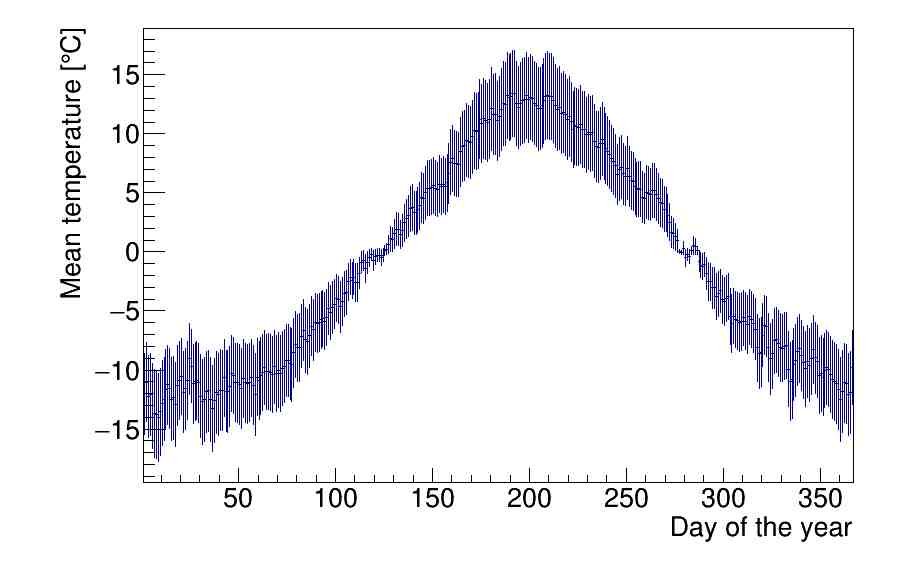
\includegraphics[width=\textwidth]{KIR_A.jpg}
        \caption{Kiruna}
    \end{subfigure}
    \begin{subfigure}[b]{0.49\textwidth}
    \centering
    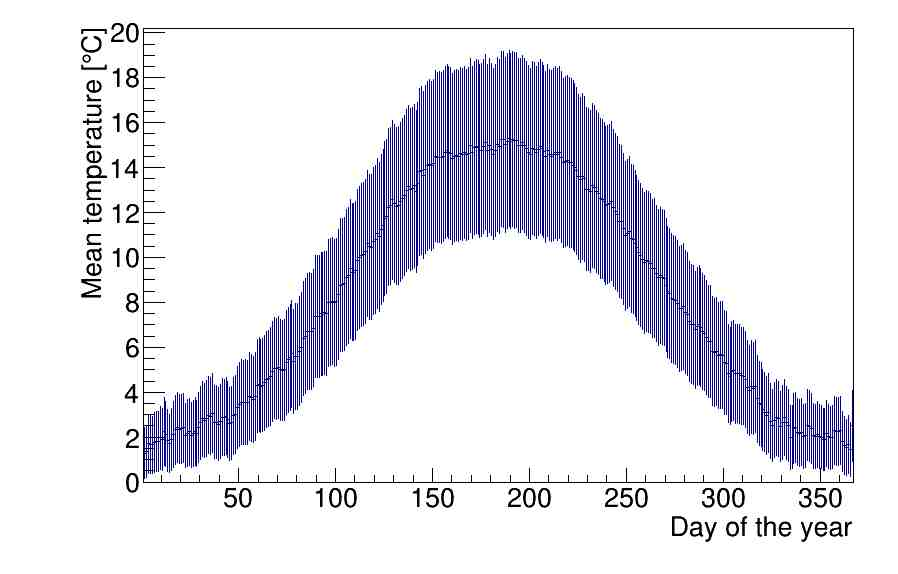
\includegraphics[width=\textwidth]{LU_A.jpg}
        \caption{Lund}    
    \end{subfigure}
    \hfill
    \begin{subfigure}[b]{0.49\textwidth}
    \centering
    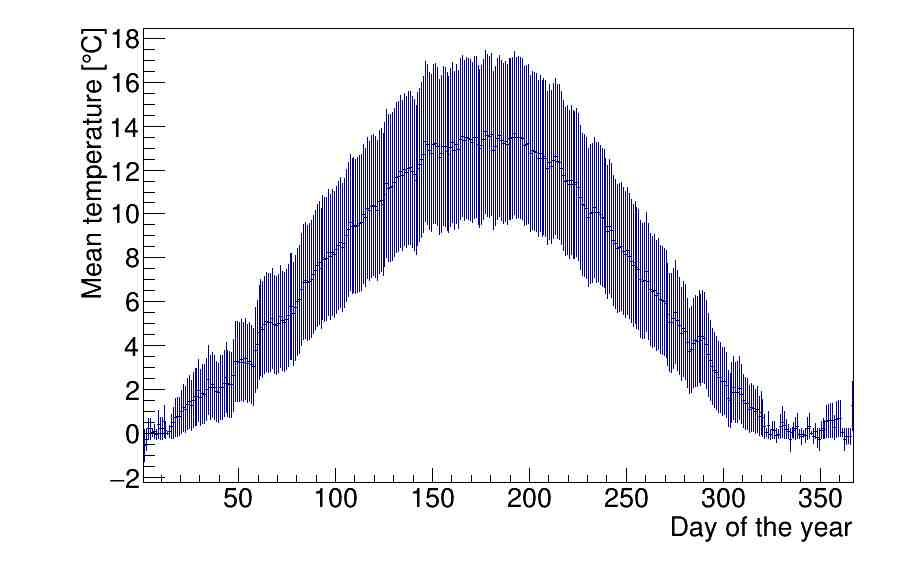
\includegraphics[width=\textwidth]{STH_A.jpg}
        \caption{Stockholm}    
    \end{subfigure}
\end{figure}




%Lund: Max: 14.3896, Min: 1.35988 
%Falsterbo: Max: 15.2263, Min: 1.98313
%Kiruna : Max: 13.4096, Min: -14.0109
%Göteborg: Max: 14.6356, Min: 1.43963
%Gävle: Max: 13.8721, Min: -2.83569
%Jönköping: Max: 12.6589, Min: -0.163235


\section{Covariance between cities}
% As an extension to the project we decided to investigate the correlation between two different cities, with possibly a time lag. To this end we implement an extra function into our \texttt{tempTrender} object. This function takes as inputs a data path for another measuring station and then plots the correlation graph between the two stations. \\
%We now present some figures showing the correlation between different cites with different time lags

For our third result we wished to study the covariance of the temperature between different cities with possibly a time lag. We made use of three cities, Lund, Falsterbo and Umeå. The covariance $Cov(X,Y)$ of two real-valued random variables $X, Y$ is formally defined as $Cov(X,Y) = E((X-E(X))(Y-E(Y))$, where $E(X)$ is the expectation of $X$. Intuitively, or as an interpretation, the covariance tells us how $X$ and $Y$ relate to each other, that is, it is the degree by which the random variables change with respect to each other. 

The way we did this was by implementing an extra function into our \texttt{tempTrender} object. This function takes as inputs a data path for another measuring station and then plots the covariance between the two. 

We show some figures of the covariance between Lund and Falsterbo. Further we show the covarriance between  Lund at different time lags.


\begin{figure}[h]
    \centering
    \begin{subfigure}[b]{0.49\textwidth}
    \centering
    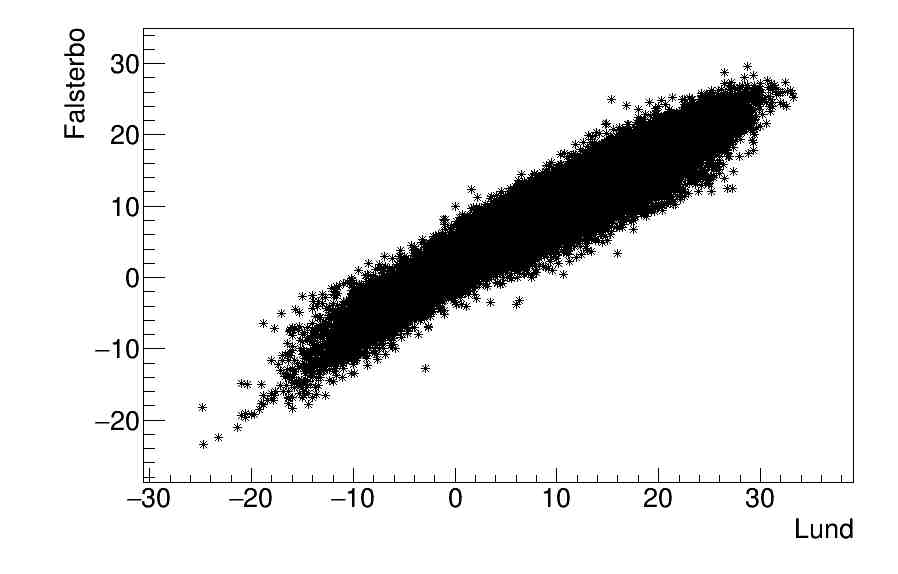
\includegraphics[width=\textwidth]{LU_FAL_E.jpg}
        \caption{Covarriance between Lund and Falsterbo}
    \end{subfigure}
    \hfill
    \begin{subfigure}[b]{0.49\textwidth}
    \centering
    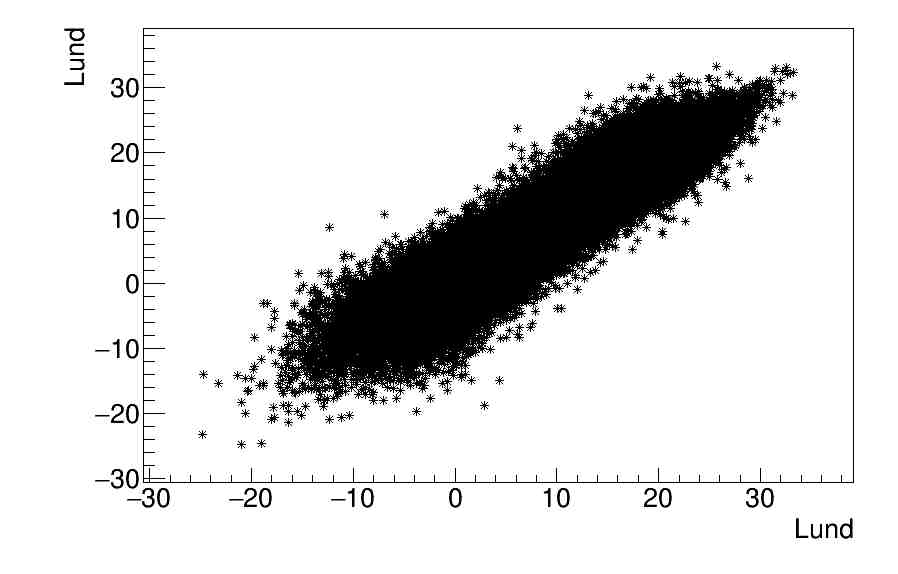
\includegraphics[width=\textwidth]{LU_LU_1D_E.jpg}
        \caption{Lund with time lag 1 Day}
    \end{subfigure}
    
    \begin{subfigure}[b]{0.49\textwidth}
    \centering
    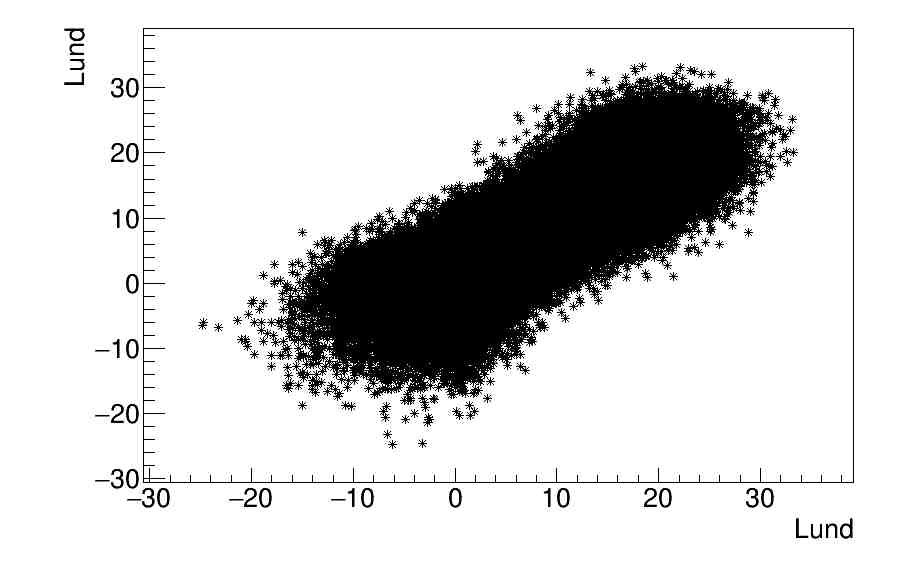
\includegraphics[width=\textwidth]{LU_LU_1W_E.jpg}
        \caption{Lund with time lag 1 Week}
    \end{subfigure}
    \hfill
    \begin{subfigure}[b]{0.49\textwidth}
    \centering
    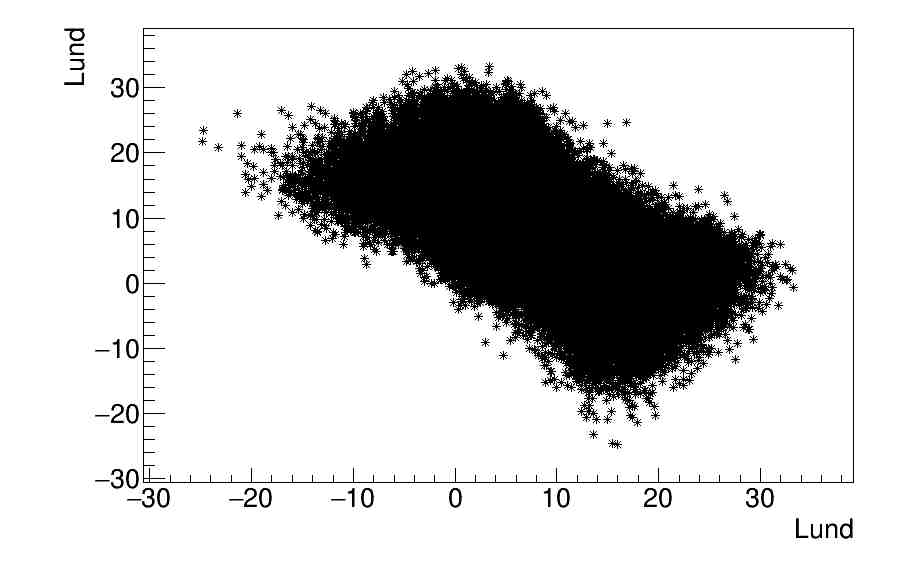
\includegraphics[width=\textwidth]{LU_LU_6M_E.jpg}
        \caption{Lund with time lag 6 Months}
    \end{subfigure}
\end{figure}

Due to the close proximity of Lund and Falsterbo we expected the covariance for Lund and Falsterbo to be fairly good. Further we should see a better correlation in the graphs with a time lag with 1 day than 1 week, while the 6 months time lag should have very week negative correlation which we see. 

\newpage


\end{document}
